% intro.tex

%In this chapter we will present our findings and evaluate what impact the added features have on a working node.
In this chapter we will present the data we have collected from our measurements and how they were taken.

While management and monitoring can be both useful and convenient, it does introduce overhead. This overhead should not have a significant impact on system performance, others citing as low as 1-2\% impact as tolerable.

Here we will verify the impact of our work on the overall throughput and performance of the software under different workloads. We will look at requests processed per second and response time distribution under typical usage patterns and some edge cases. 

We will first look at single node performance, with and without our modifications.
Next we will try verifying that performance scaling is intact. For Voldemort, near linear scaling of throughput is expected when adding worker nodes to the cluster.
Lastly we will look at performance during a automatically triggered rebalance under load.

\section{The tests}
All tests are run on a clean cluster instance, with a warm up period loading data into the database. All tests are run three times, with the average score used.

Test0:

100\% read ?
100\% read no mod ?

99\% 1\% read/update ? read/write?
99\% 1\% read/update ? read/write? no mod

1\%/99\% read/write ?
1\%/99\% read/write ? no mod

linear scaling:
100\% read ? 2 nodes
100\% read no mod ? 2 nodes

99\% 1\% read/update ? read/write? 2 nodes
99\% 1\% read/update ? read/write? no mod | 2 nodes

These are the most realistic workloads for Voldemort, as a high volume read only service and about 98-99\% read to write/update.

rebalance:
Just monitor request rate during a rebalance.
Remember to somewhat record size of data set.

\begin{center}
\begin{table}[h]
	\begin{tabular}{|c|c|c|c|c|l|}
		\multicolumn{1}{c}{Test case} & 
		\multicolumn{1}{c}{Node \#} &
		\multicolumn{1}{c}{Cluster size} &  
		\multicolumn{1}{c}{read \%} & 
		\multicolumn{1}{c}{write \%} & 
		\multicolumn{1}{c}{state} \\
		\hline

		TC1.1 & 1 & 1 & 95 & 5 & official \\
		TC1.2 & 1 & 1 & 95 & 5 & modified \\
		\hline
		TC2.1 & 2 & 1 & 95 & 5 & official \\
		TC2.2 & 2 & 1 & 95 & 5 & modified \\
		\hline
		TC3.1 & 3 & 1 & 95 & 5 & official \\
		TC3.2 & 3 & 1 & 95 & 5 & modified \\

		\hline
	\end{tabular}
	\caption{Test case setup. Official/modified is shorthand for whether we will be using original or our source code for this test.}
	\label{tbl:testcases}
\end{table}
\end{center}

% figures.tex


\begin{figure}[h]
    \centering
    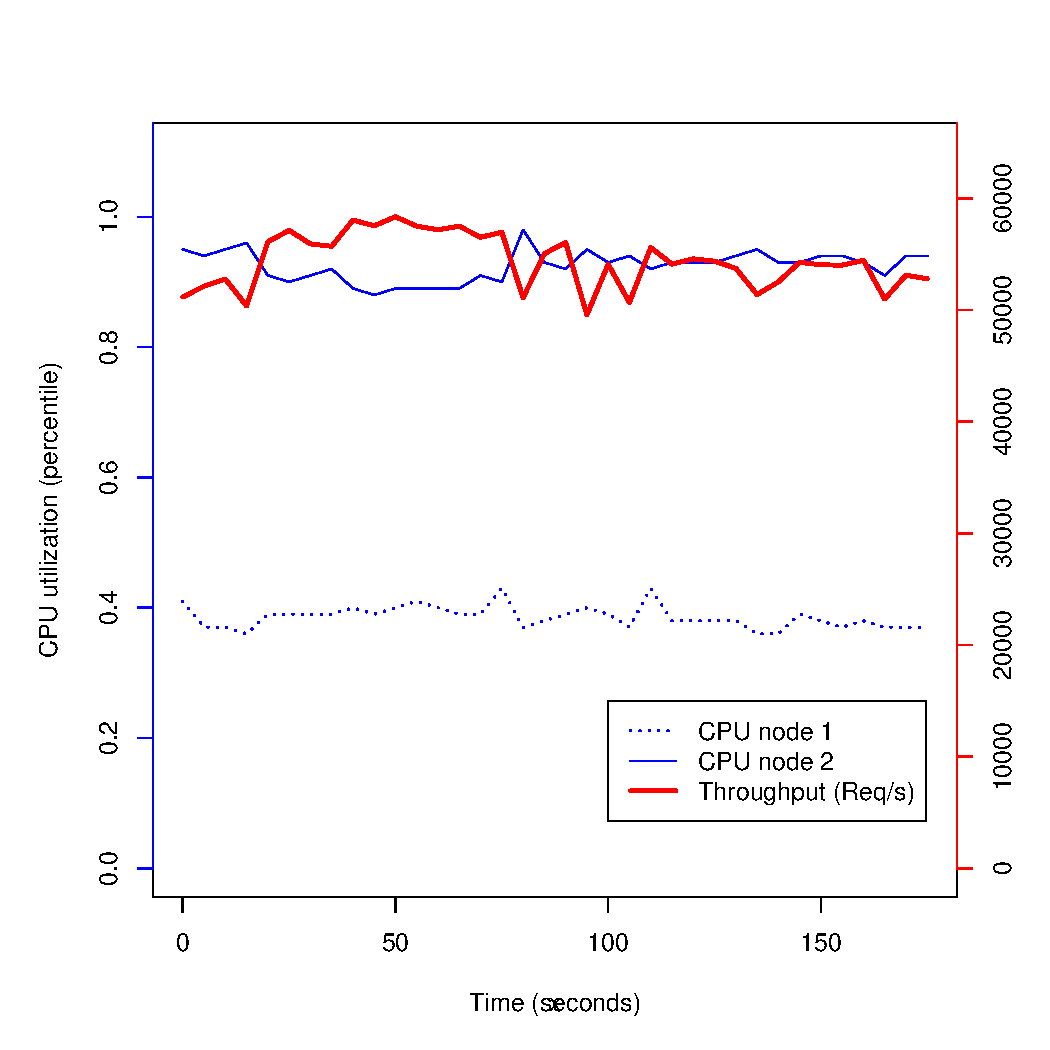
\includegraphics[width=1.2\textwidth]{results/baseline_plot}
    \caption{Baseline}
    \label{fig:baseline}
\end{figure}

\begin{figure}[h]
    \centering
    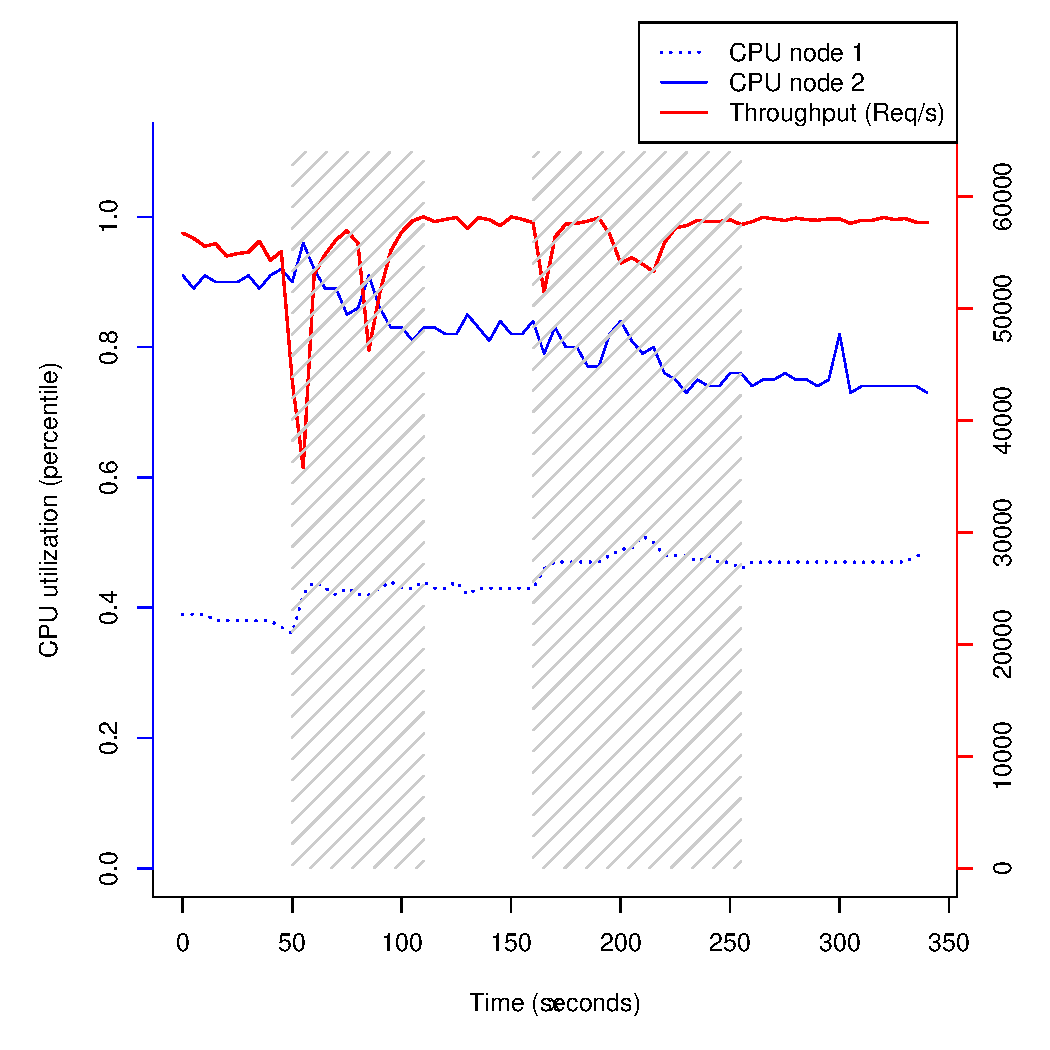
\includegraphics[width=1.2\textwidth]{results/adaptive_plot}
    \caption{Moving of 3 partitions from a struggling node (Node )}
    \label{fig:adaptive}
\end{figure}




\section{Experiments}
\subsection{Setup}
\subsubsection{Benchmark tool}
We use Voldemorts provided benchmark tool to send data to our cluster. The program is heavily based on the work by Yahoo Cloud Serving Benchmark. This allows us to generate different types of workloads, request loads and number of sending threads. We also had to do some modifications to get a running average, instead of a total average.

We parse most of the logs in python to transform the data into something useful. In some cases we also have to manually put the data together.
For analysis, we mainly use \texttt{R}\cite{Rproject} with extensive use of the \texttt{Hmisc}\cite{Hmisc} library. Our Rscripts can be found in our project on github\cite{githubproject}. Most of the diagrams in this chapter has been generated with \texttt{R}.

An example run with the benchmark tool could be:
\begin{lstlisting}[language=bash]
read_percent=95
write_percent=5
metric=histogram # [summary|histogram]
ops=1 000 000 # total requests to run
threads=54
recordcount=1000000 # records to insert during warmup
valuesize=1024 # bytes per record

voldemort-performance-tool.sh --threads $threads --metric-type $metric 
--ops-count $ops --url $url --value-size $valuesize 
--store-name $store --record-count $recordcount $@
\end{lstlisting}

These are also the settings we used for most of our tests.

\subsubsection{Hardware}
We have 4 computers involved in these experiments:

\begin{enumerate}
	\item Hackintosh: Intel Core i7 2.5GHz Quad Core  16 GB Memory 250GB SSD
	\item MacBook Pro: Intel Core i7 2.6 GHz Quad Core 8 GB Memory 250GB SSD
	\item MacBook Pro: Intel Core i5 2.5 GHz Dual Core 8 GB Memory 120GB SSD
	\item Mac Mini: Intel Core 2 Duo 2.4 GHz Dual Core 8 GB Memory 250GB SSD
\end{enumerate}

In addition we use a D-Link Dir-655 gigabit router for networking.

\subsubsection{Software}
All computers run Apple OS X 10.9.2 operating system. 

\subsection{Initial benchmarking}
In this part we want to investigate how our computer and cluster behaves in various scenarios. We will in all experiments use a workload of 95\% read and 5\% write requests as is common on a typical social website. Each data entry is 1kB. 


\subsubsection{Response time distribution}
We want to establish a baseline for how each individual node performs with regards to servicing requests. In this experiment we will setup a single node Voldemort instance, and measure the service time over a given number of requests. We will run this test with both our ZooKeeper implementation and the original Voldemort code, sending queries as fast as possible.

We expect similar results between the nodes, as all nodes will run at maximum capacity. We also expect the majority of these requests to be serviced in under 1 ms as found by Rabl et al\cite{Rabl:2012:SBD:2367502.2367512}.

\subsubsection{Throughput of single nodes}
We also want to get an idea of each individual nodes ability to service queries. To test this we will again run single node clusters and send requests as fast as possible. The throughput is measured for 1 million requests, each for values of size 1024 bytes.

%%% This is for evaluation I think?
%With our workload and entry size we have a theoretical limit of around 60 000 requests per second as this is equal to 125MB or 1Gbit data per second. We expect the 4 cores of the i7 to be able to serve up to 60 000 requests, while the two computers will perform considerably worse. 

\subsection{Experiments on the cluster}
In this part of the experiments we have a look at how a cluster consisting of several nodes performs. We will explore different scenarios both with and without rebalancing.

\subsubsection{Baseline}
In this experiment we want to establish a baseline for how a cluster behaves under load. We have both MacBooks sharing 16 partitions. We define node 1 to be the Core i7 MacBook and node 2 to be then Core i5 Macbook.  We use the Hackintosh for generating traffic. 

We expect node 1 to be able to serve its requests with ease while node 2 will struggle with near 100\% utilization of the CPU. As this is not an optimal work distribution we expect measured throughput to be lower than under optimal conditions. As in the case with the initial benchmarks, we will run the tests both on our ZooKeeper implementation and the original Voldemort project. 

\subsubsection{Adaptive cluster experiment}
In this experiment we want to see how the cluster behaves when we allow a struggling node to move partitions over on a node under less stress. Node 1 and 2 are set up the same way as in the baseline experiment. A struggling node is defined as a node running at less than 20\% idle CPU.

We expect throughput to be lower during the rebalance phase, but overall we will see an increase in performance over time as we gain a more optimal distribution of partition. 

We will again run the experiment on both our implementation and the original Voldemort implementation to see if there is any major differences in performance. On the original implementation we trigger rebalances manually until we reach a state where no node is stressed. 

After viewing the results we found a severe bug in our ZooKeeper implementation. Which led us to redo this test on our implementation. More on this in the results section. We chose to include the incorrect result for completeness. 


\subsubsection{Mini and slowpro with fastpro to the rescue}
In this experiment we will utilize all our features by adding a node to a already struggling cluster and automatically move partitions to alleviate the existing nodes. We will have a cluster consisting of the Mac Mini and i5 MacBook Pro and we will add the i7 Macbook Pro during the experiment. 

We expect the system to perform poorly during the initial phase as both computers will be running at near max capacity. After we add third computer and move the first partition the performance should increase. As the system migrates more partitions away from the struggling nodes the overall performance should keep increasing. 

\subsubsection{Partitions containing lots of data. See how much throughput is affected. Different rebalance strategies}





\section{Results}

\subsection{Initial benchmarking}
Below we present our results

\begin{figure}[h]
    \centering
    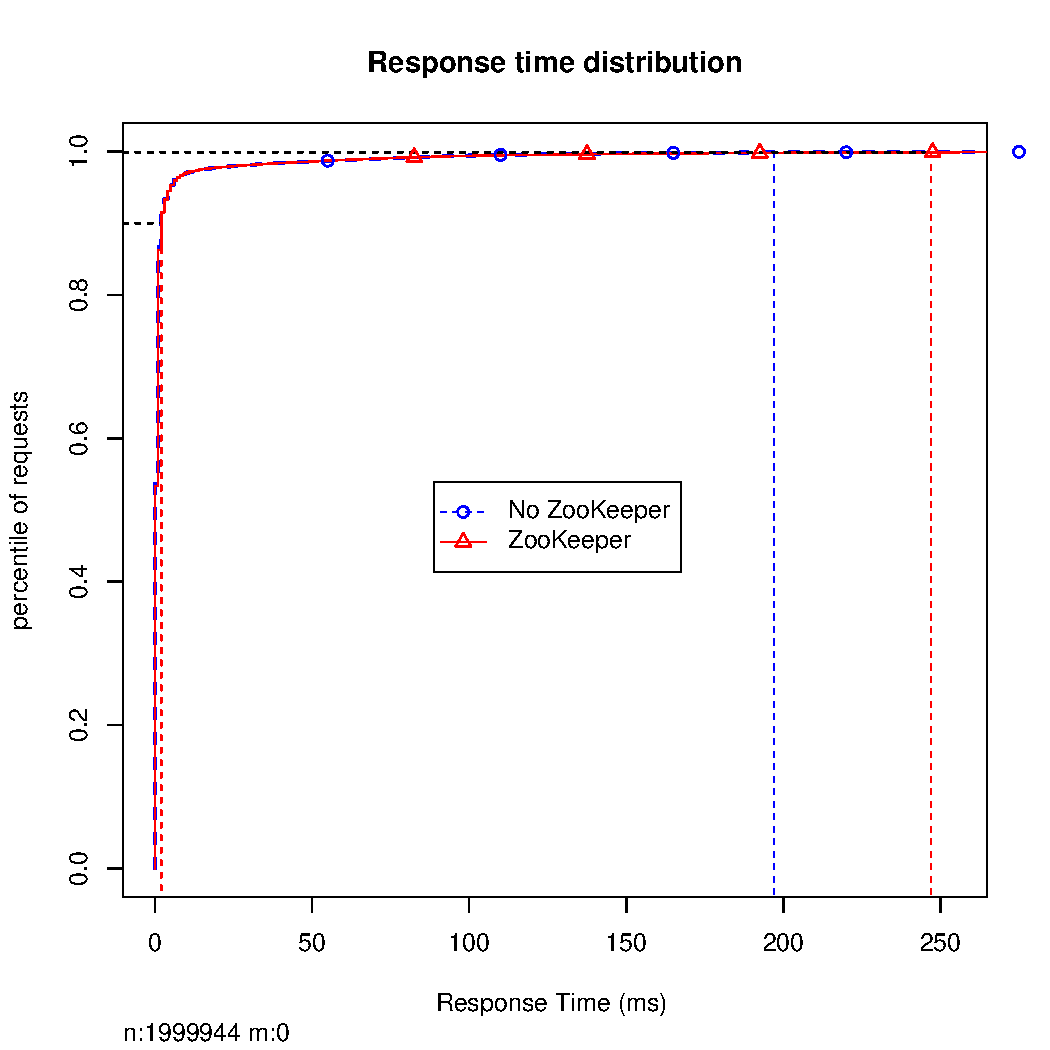
\includegraphics[width=0.8\textwidth]{results/distribution/distribution_macmini}
    \caption{Response time distribution Core 2 Duo Macmini}
    \label{fig:dist_knut}
\end{figure}

\begin{figure}[h]
    \centering
    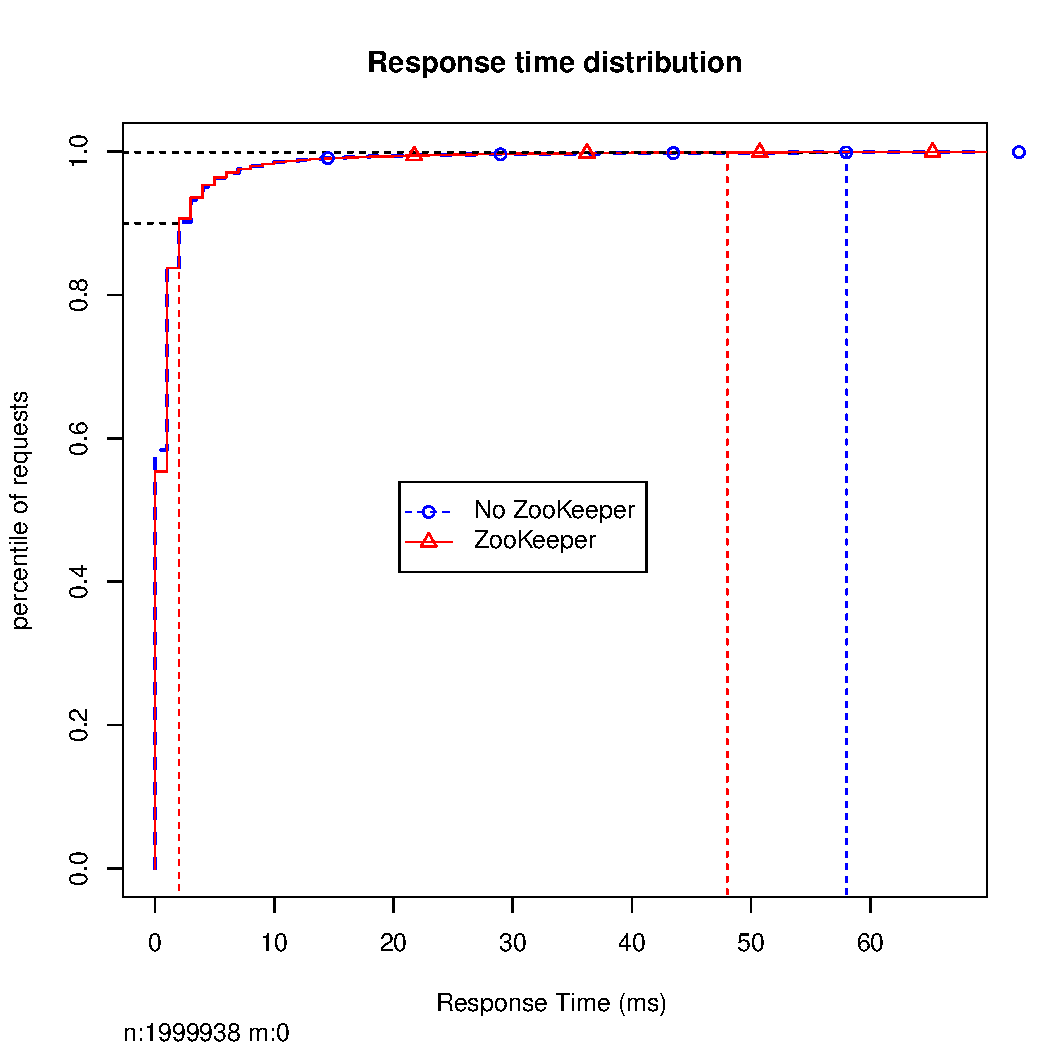
\includegraphics[width=0.8\textwidth]{results/distribution/distribution_knut}
    \caption{Response time distribution i5 MacBook}
    \label{fig:dist_knut}
\end{figure}

\begin{figure}[h]
    \centering
    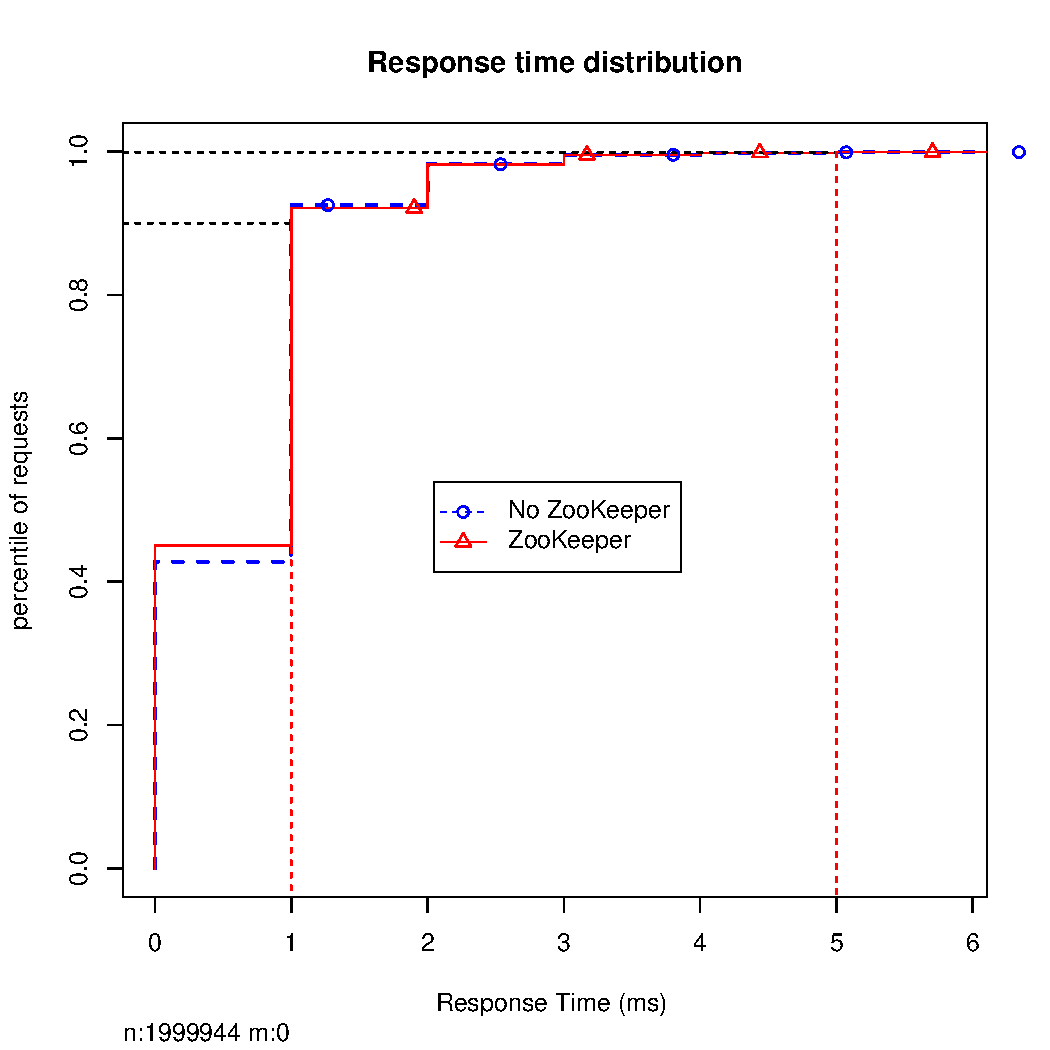
\includegraphics[width=0.8\textwidth]{results/distribution/distribution_eivind}
    \caption{Response time distribution i7 MacBook}
    \label{fig:dist_knut}
\end{figure}








